\section{Evaluations}

There were a myriad of analyses we performed in order to test the efficacy of an ngram-based engine as described in the previous section. This section looks at how our model responds to some of the challenges we mentioned in section \textbf{1.SOMETHING} and discusses the interesting results produced. Some of the main questions that we hoped to answer were as follows: 
\begin{itemize}
  \item How well did our placeholders perform?
  \item How does the model perform for smaller datasets?
  \item Does training separate models for different roles improve our accuracies?
\end{itemize}

 We first describe our data, and then analyze the general trend we observed when implementing placeholders. Next, we outline how our analyses show that across both dimensions of time and length, the NLP algorithm is resistant to data scarcity. Furthermore, we showed how breaking up the configurations by router roles gave us unexpected results.

\section{Configuration Data}

We applied our framework to Cisco configurations of core, border, and distribution routers from three large university networks(Table~\ref{tab:datasets}). The figure below shows us the distribution by size for configurations from all universities combined. Additionally, we were also able to get extensive data from University A's version control histories. This allowed us to perform some tests based on snapshots sampled across time. We used monthly time intervals for such tests.

\begin{table}
    \small \centering
    \begin{tabular}{ | c | c | c | c |}
    \hline
        {\bf Univ.} & {\bf No. of Configs} & {\bf Total Lines} & {\bf Avg
    Lines} \\ 
    \hline
    A & 35 & 73K & 2.1K \\ 
    B & 26 & 61K & 2.3K \\ 
    C & 24 & 67K & 2.8K \\ 
    \hline
    \end{tabular}
    \caption{Configurations used in our evaluation}
    \vspace{-1em}
    \label{tab:datasets}
\end{table}

\begin{figure}[H]
	\centering
	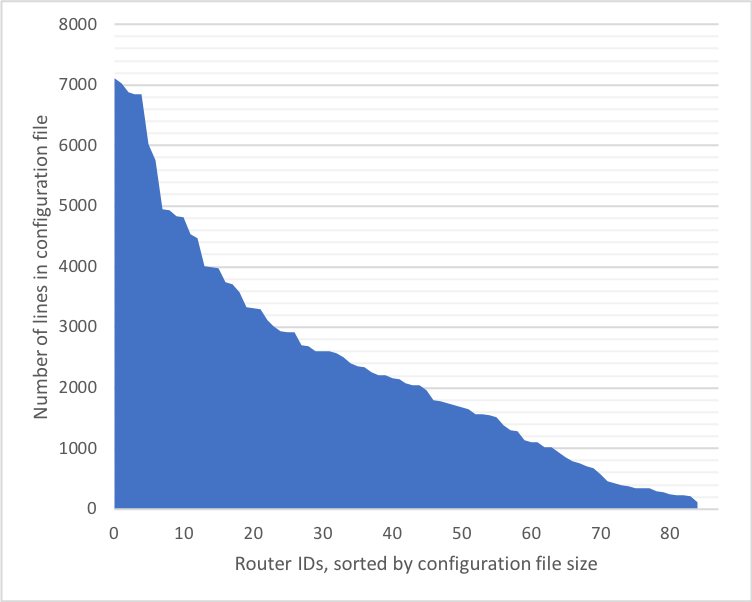
\includegraphics[width=5in]{config_sizes.png}
	\caption{Our data has a good mixture of long and short configurations}
\end{figure}

\subsection{Testing Methodology}

To test the accuracy of our model, we perform Leave One Out (LOO) Cross Validation. This form of cross validation involves using one observation as the validation set and the remaining observations as the training set. This is repeated for all combinations of training sets, allowing every observation to act as a validation set. For our analyses an observation could be one set of configurations or just one device configuration depending on the test. For example, for our analyses on length of histories, a validation set is comprised of all device configurations for a given month whereas for an analysis on the number of devices, the validation set is the configuration of one routing device.\\

For a single test, we "walk through" rebuilding the validation set token-by-token, starting from the first keyword. For every line we do not predict the first token but invoke the model for every subsequent token. Figure 4 shows us what this test conceptually looks like. On the left handside we have a configuration that is being built using the model and on the right the complete original configuration. Consider the line pointed to by the red arrow. We assume that the first keyword ("ip") is given to us. We then use the model to generate three suggestions
\footnote{The code completion papers we read considered a prediction to be correct if it appeared within the top three to five suggestions. Accurately predicting the correct token within one suggestion every time can be extremely difficult for any code completion system, which is why developers give themselves some leeway when assessing a model's accuracy}
for the next token and check against the original configuration see whether the correct token ("address") was within this list of suggestions. The next step would be to consider both "ip" and "address" to generate suggestions for the third token. As we are using trigrams, we do not consider more than two previous tokens at a time. We use the ratio of the number of correct predictions to the number of model invocations as a measure of the model's accuracy.\\

\begin{figure}[H]
	\centering
	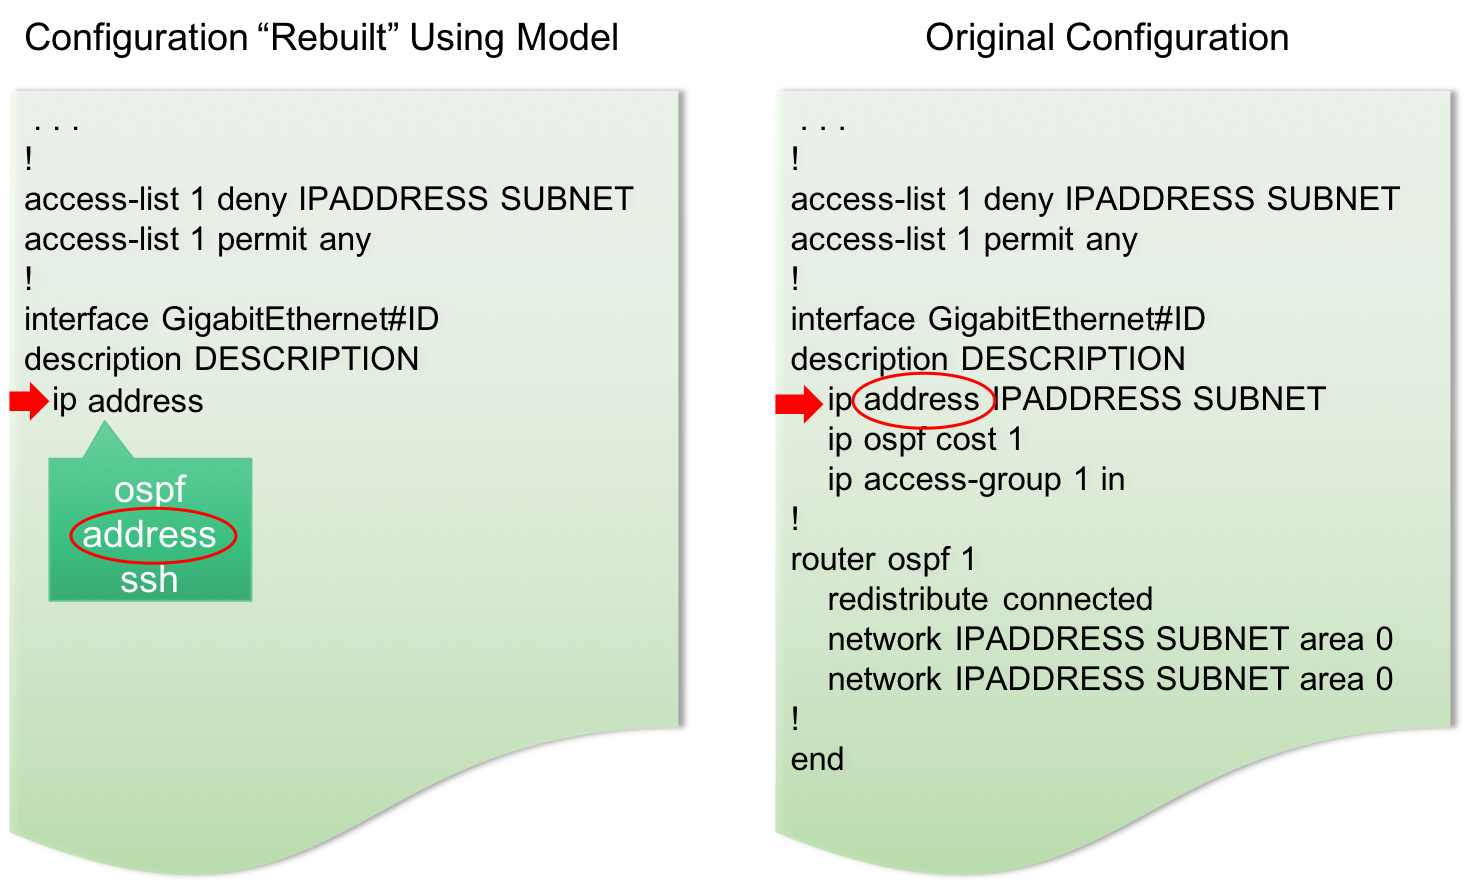
\includegraphics[width=5in]{validation_example.png}
	\caption{A visualization of how a validation test is carried out}
\end{figure}


 
\begin{figure}[H]
	\centering
	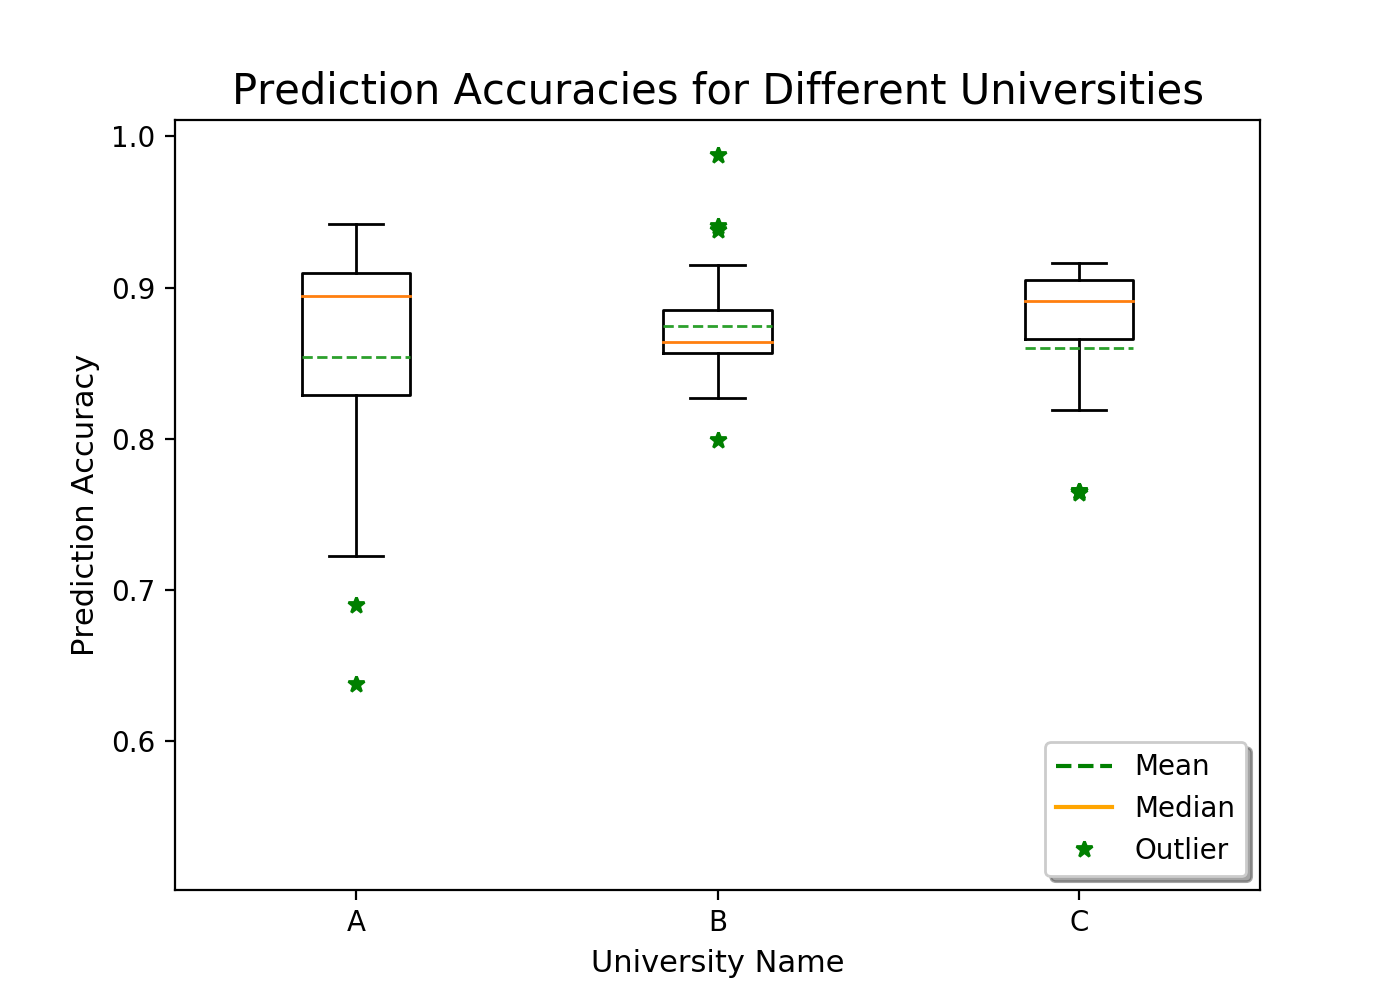
\includegraphics[width=5in]{uni_analysis.png}
	\caption{Overall accuracy of the model for each set of university configurations used as the validation set.}
\end{figure}

In Figure 5, we show the overall accuracy of our model. The the x-axis shows the name of the three anonymized universities used, and prediction accuracies on the y-axis. The box plot is supposed to highlight the average (green dotted line), median (orange line) and upper ($Q_U$) and lower quartiles ($Q_L$). The box itself marks the Inter Quartile Range (IQR). The outliers (green stars) are all the data points that lie outside $Q_L - 1.5*IQR$ and $Q_U+1.5*IQR$.\\

Initially, without any preprocessing and subnet removal, we observed a maximum accuracy of 85\% and an average of 65\%. Our results in the figure above are after preprocessing the data and we now see accuracies as high as 93\%, and an average of 81\%. These results are very promising as we see a significant jump in accuracy from simple refinements to the model. More placeholders would improve accuracies even further but with diminishing returns.

\subsubsection{Placeholders}

\begin{figure}[H]
	\centering
	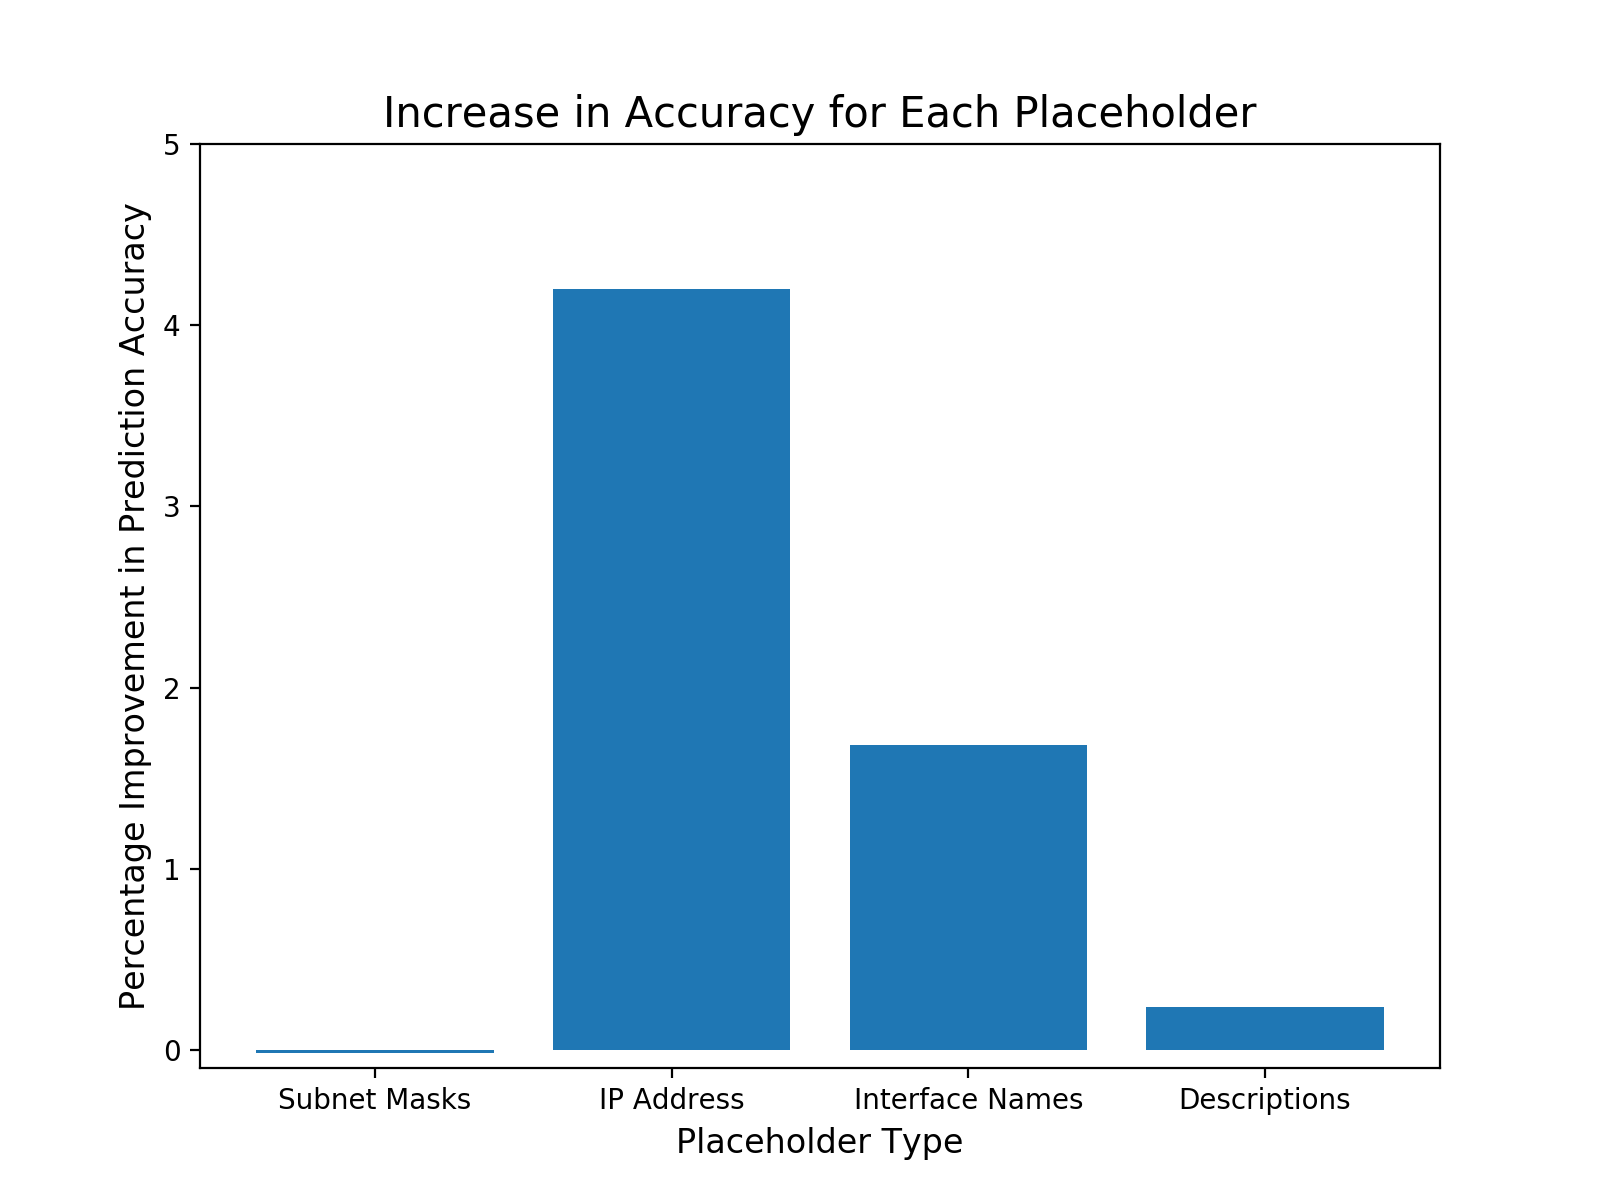
\includegraphics[width=\textwidth]{placeholders.png}
	\caption{Effect on Accuracy by Every Placeholder}
\end{figure}

Generally, we see an improvement when placeholders are used to substitute certain keywords. As the graph shows, the biggest jump in accuracy is accomplished by using IP address placeholders. This is expected, as configurations are bound to consist of a number of unique IP addresses which it makes it extremely difficult to predict which one is going to be used. Other tokens, for example subnet masks, tend to be much more homogeneous (usually a handful of subnet masks are repeatedly used across a network). As placeholders were resulting in diminishing returns, due to time constraints, we decided to go ahead with the ones we had implemented. We leave additional placeholders as a possible future extension.


\subsubsection{Length of Histories}

\begin{figure}[H]
	\centering
	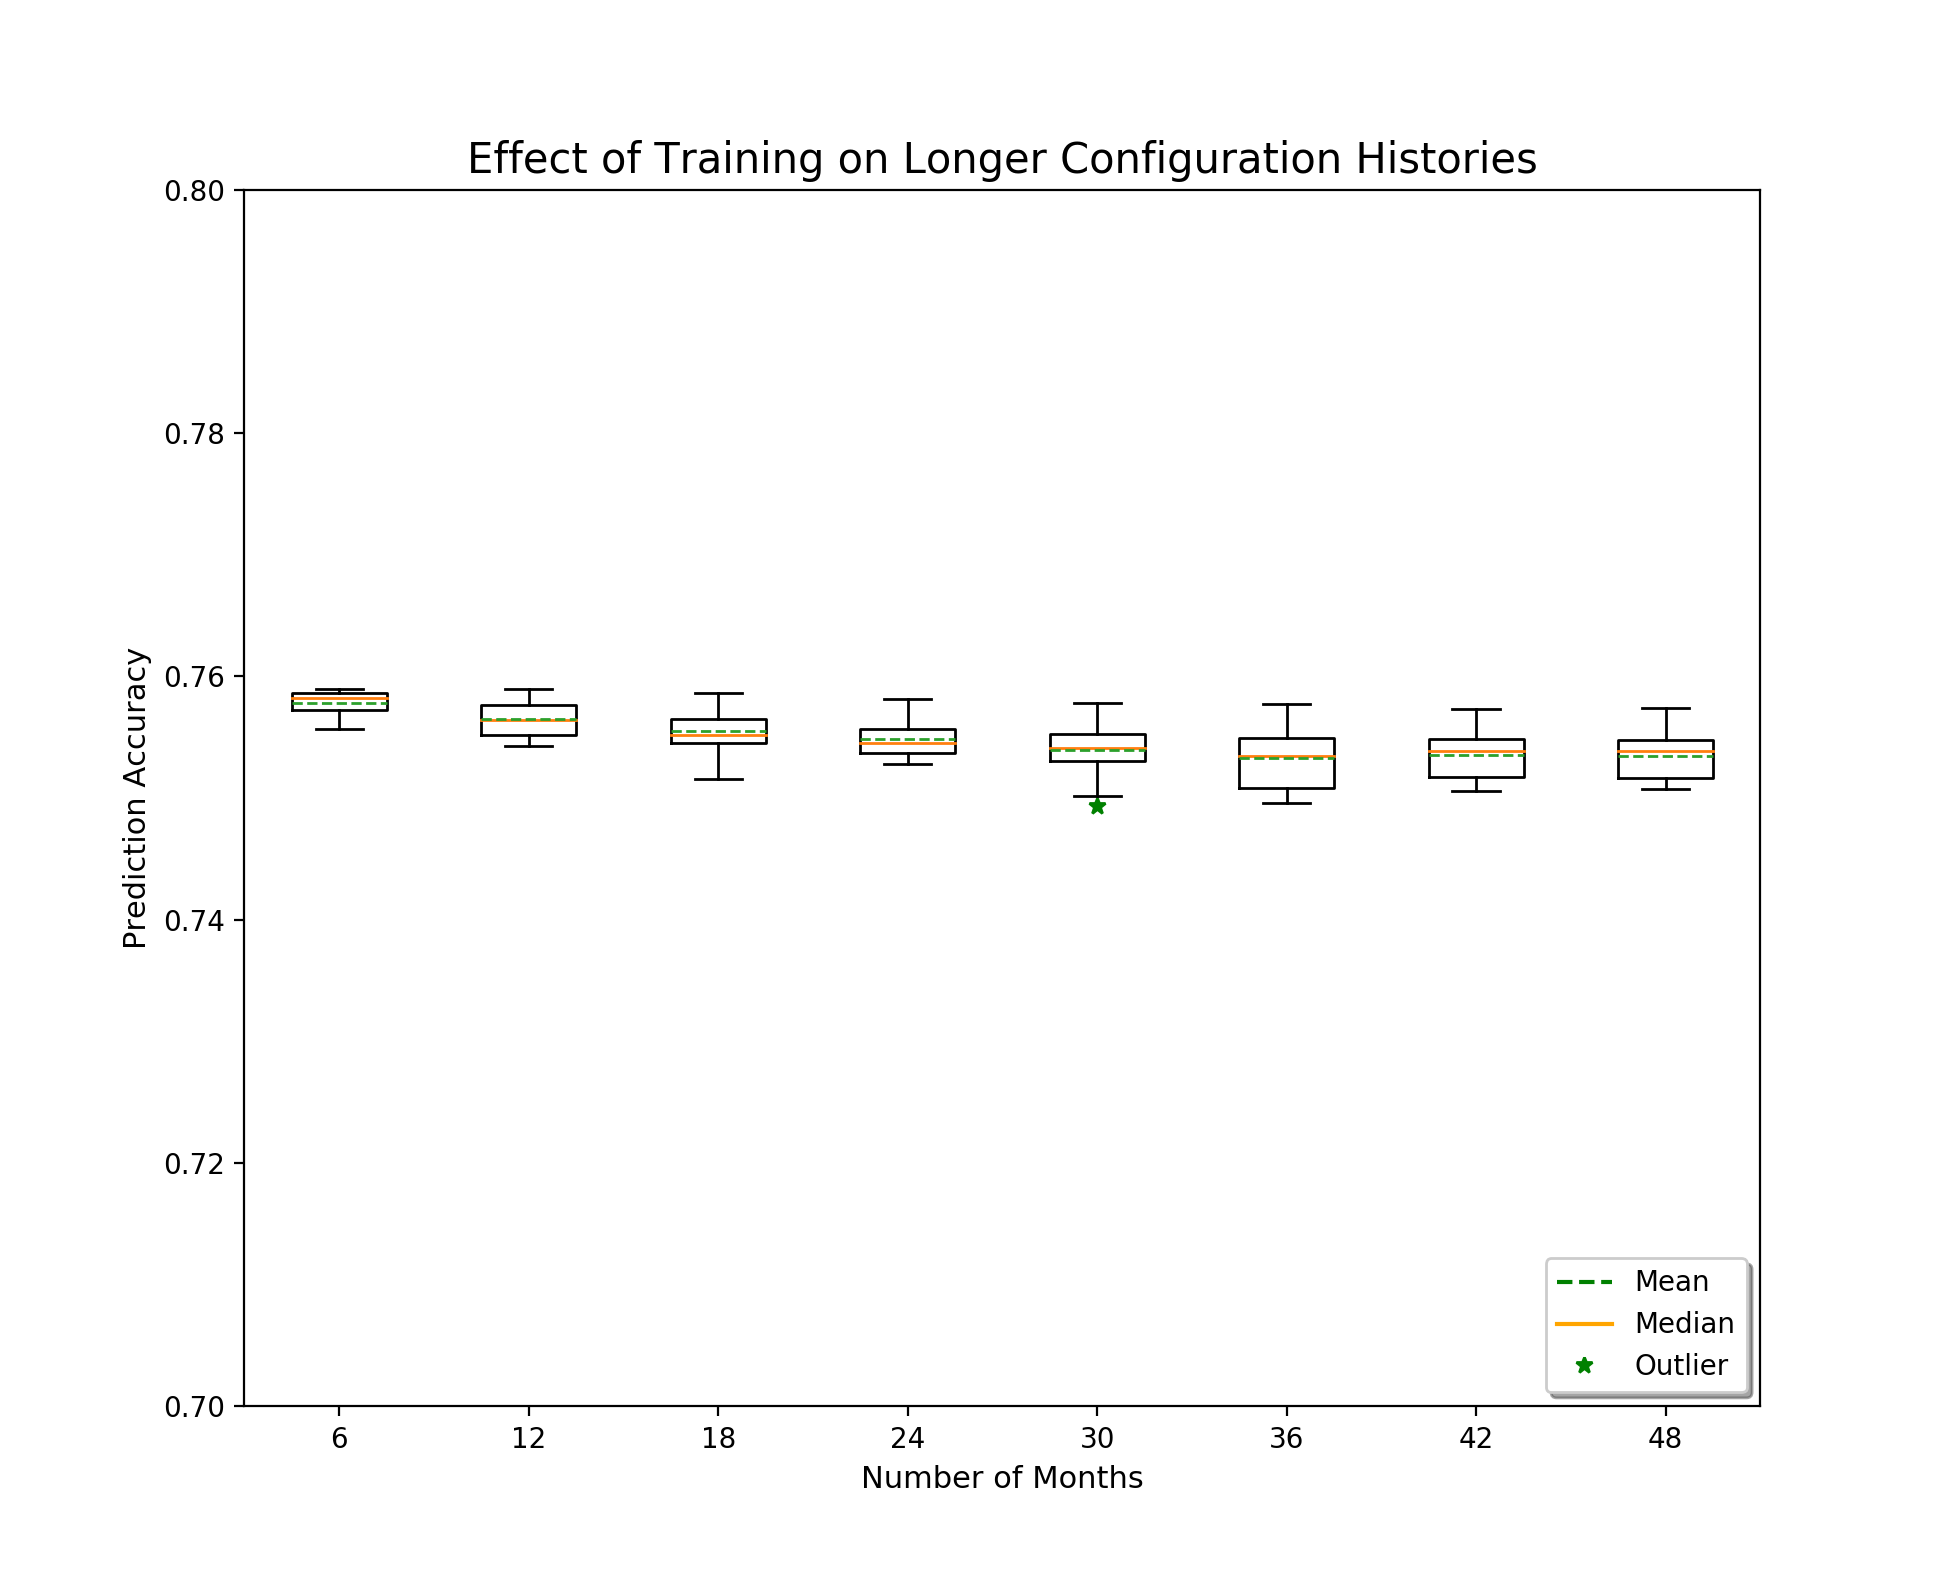
\includegraphics[width=\textwidth]{time.png}
	\caption{Longer histories may not result in higher accuracies.}
\end{figure}

As we had extensive data from University A's version control system, we analyzed the effect of selecting configurations across time on prediction accuracies. The x-axis of the graph shows the number of months we chose to train on. As is apparent from the image, if we train on longer configuration histories our accuracies stay about the same. In fact, we see a slight decrease which may be attributed to the variation introduced by the increased data points. We do expect some change in the configurations over time as the university networks evolve. However, these changes tend to be small and homogeneous as the analyses from from ~\cite{Kim} inform us. Thus, our model does not need to consider configurations across 4 years for this university.

\subsubsection{Number of Devices}
\begin{figure}[H]
	\centering
	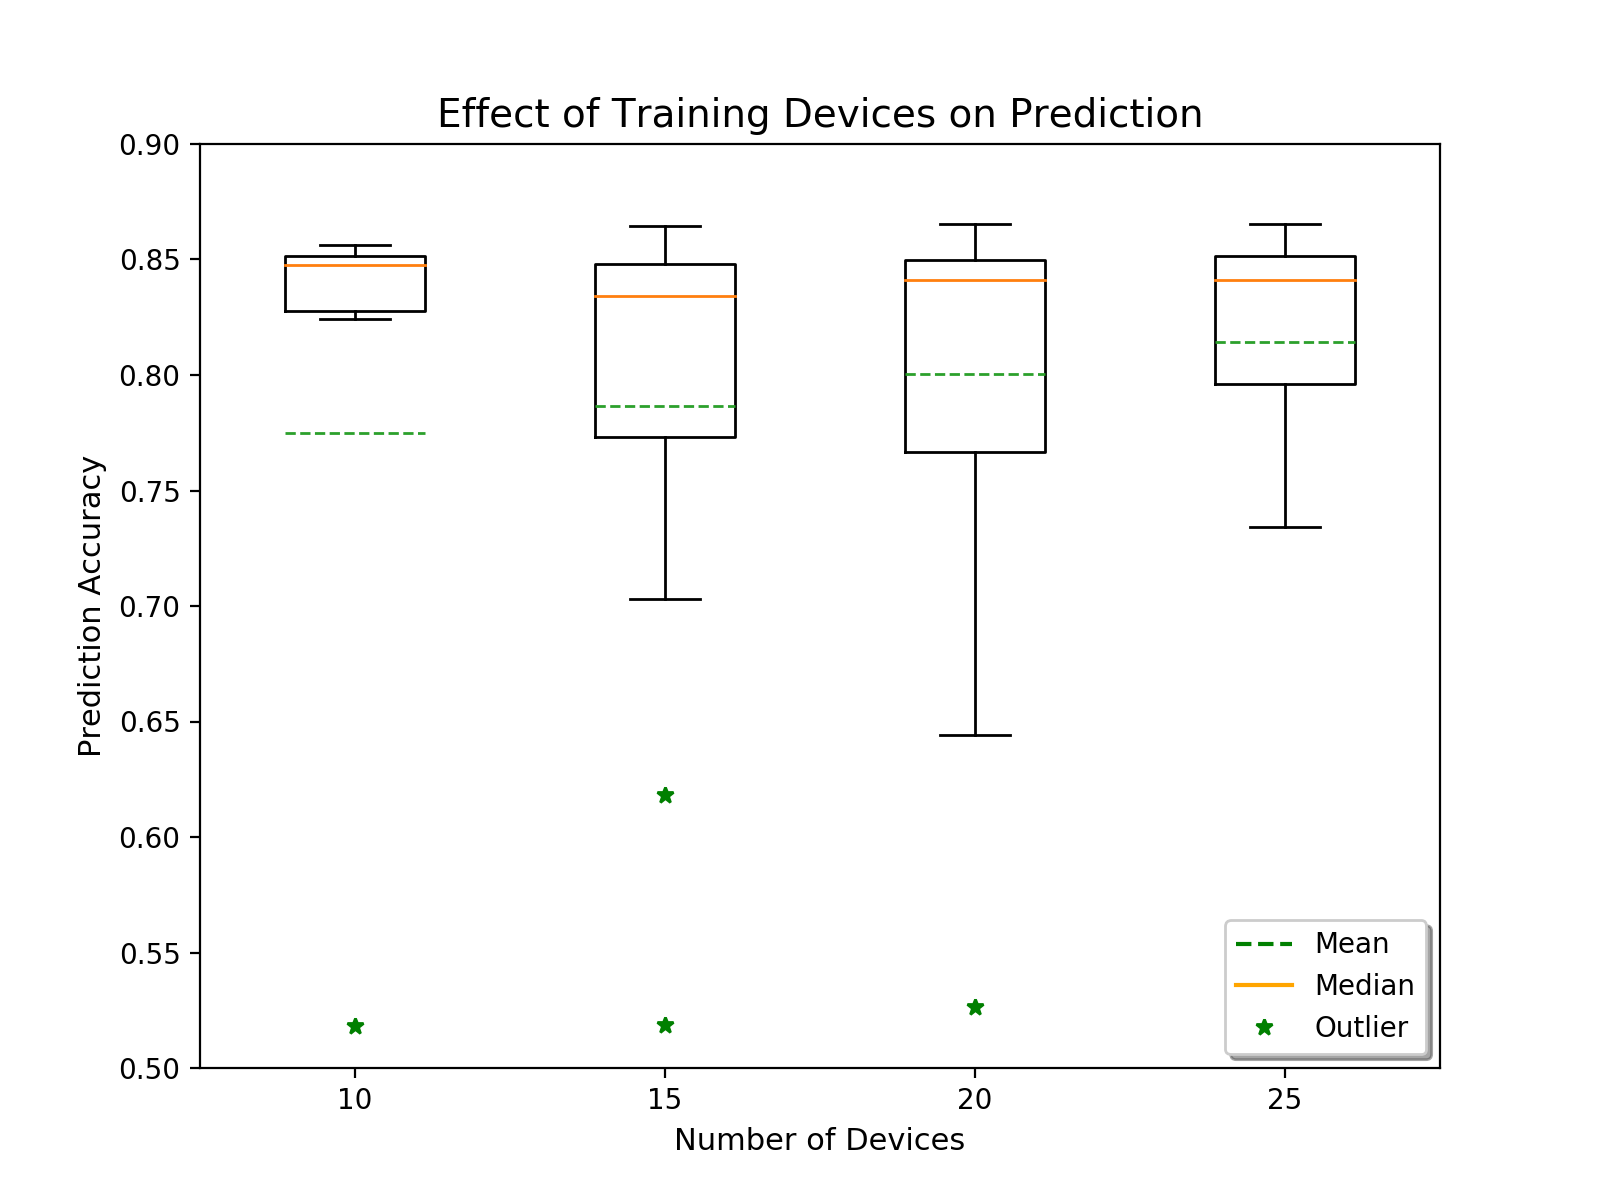
\includegraphics[width=\textwidth]{device_analysis.png}
	\caption{Training across more devices does improve accuracy to a certain point.}
\end{figure}

As we add configurations from more devices to our training set, we see a slight increase in accuracy before it starts to give us diminishing returns. This may mean that the model has already seen most of the tokens that are often used by network operators. Every additional device contributes less to the overall model prediction set. In practice some devices being added may be different from the rest of the network, causing them to act as outliers which would be affecting our averages.

\subsubsection{Role-Based}

\begin{figure}[H]
	\centering
	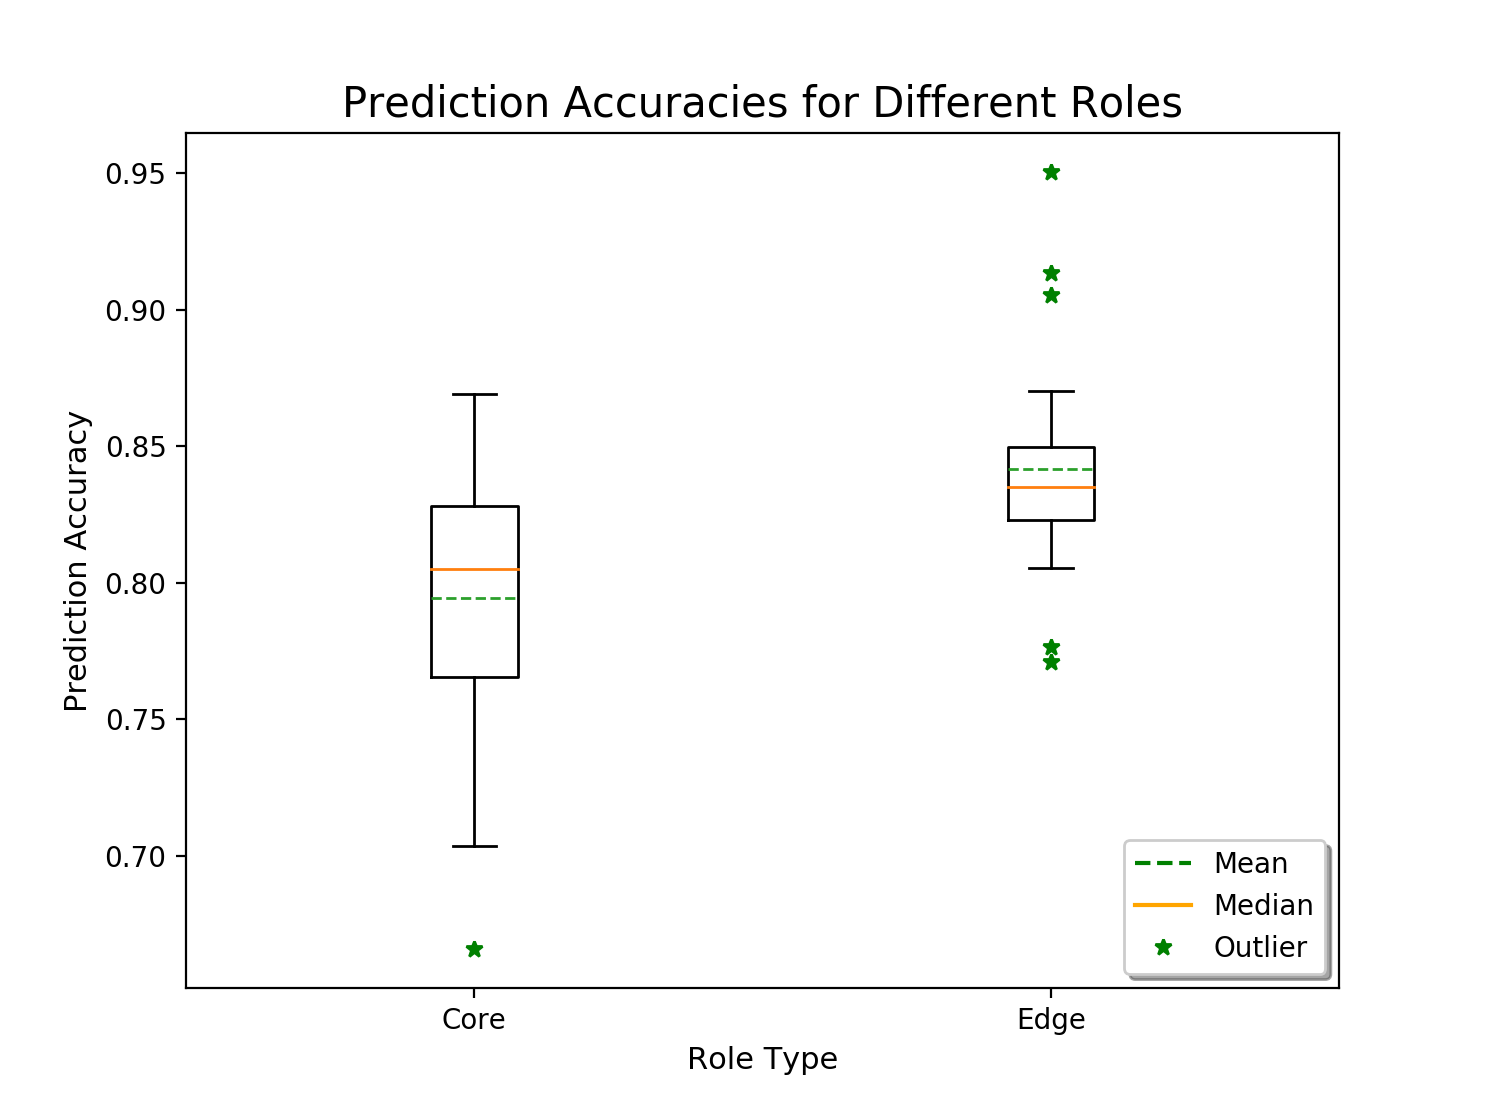
\includegraphics[width=\textwidth]{roles.png}
	\caption{Accuracies of models were trained on core and edge routers only, with the first boxplot showing the combined training set}
\end{figure}

Splitting by roles did not result in an improvement in accuracy like we expected. There are a few factors that could be contributing to this result. It might be possible that there is not much variation in the two roles to begin with. We were assuming that the suggestions generated by the "combined" version would contain the tokens for both edge routers and core routers which would reduce the chances of the correct one cropping up in the top 3 suggested tokens. However, the results show that after separation, edge routers did not fare any better and core routers actually did worse. We also believe that this may be a problem of the labels/roles being coarsely defined as we were relying on the names of the routers to separate them. It is entirely possible that network operators may be labeling the routers as a rough approximation of their intended roles. Thus researchers may need to figure out a more fine grained way about dividing them.

